% ============================================================
%  فایل نمونه جامع LaTeX فارسی-انگلیسی
%  کامپایلر: XeLaTeX
%  هدف: تست تبدیل به MDX
%  نویسنده: نمونه تست
%  تاریخ: ۱۴۰۴
% ============================================================
\documentclass[12pt,a4paper,twoside]{book}

% ---------- صفحه‌بندی ----------
\usepackage[
  top=2.5cm, bottom=2.5cm,
  inner=3cm, outer=2cm,
  headheight=15pt
]{geometry}

% ---------- فونت و زبان (پایه) ----------
\usepackage{fontspec}

% ---------- رنگ ----------
\usepackage[dvipsnames,svgnames,x11names]{xcolor}
\definecolor{PrimaryBlue}{HTML}{1A73E8}
\definecolor{AccentTeal}{HTML}{00897B}
\definecolor{AccentOrange}{HTML}{FB8C00}
\definecolor{LightBG}{HTML}{F5F7FA}
\definecolor{DarkText}{HTML}{212121}
\definecolor{ProofBG}{HTML}{FFFDE7}
\definecolor{TheoremBG}{HTML}{E3F2FD}
\definecolor{ExampleBG}{HTML}{E8F5E9}
\definecolor{WarningBG}{HTML}{FFF3E0}
\definecolor{SidebarGray}{HTML}{ECEFF1}

% ---------- ریاضی ----------
\usepackage{amsmath,amsthm,amssymb,mathtools}
\usepackage{unicode-math}

% ---------- جدول ----------
\usepackage{booktabs,tabularx,longtable,multirow,colortbl,array}
\usepackage{rotating} % جدول افقی (landscape)

% ---------- تصویر و شناور ----------
\usepackage{graphicx,float,wrapfig}
\usepackage[font=small,labelfont=bf,labelsep=period]{caption}
\usepackage{subcaption}

% ---------- جعبه‌های رنگی ----------
\usepackage[most,skins,breakable]{tcolorbox}

% ---------- نمودار ----------
\usepackage{tikz}
\usetikzlibrary{
  arrows.meta,calc,positioning,shapes.geometric,
  decorations.pathreplacing,backgrounds,fit,
  mindmap,trees,shadows,chains,matrix
}
\usepackage{pgfplots}
\pgfplotsset{compat=1.18}
\usepgfplotslibrary{fillbetween,statistics,colorbrewer}

% ---------- کد ----------
\usepackage{listings}
\lstset{
  basicstyle=\small\ttfamily,
  backgroundcolor=\color{LightBG},
  frame=single,
  rulecolor=\color{PrimaryBlue!40},
  breaklines=true,
  numbers=left,
  numberstyle=\tiny\color{gray},
  keywordstyle=\color{PrimaryBlue}\bfseries,
  commentstyle=\color{AccentTeal}\itshape,
  stringstyle=\color{AccentOrange},
  showstringspaces=false,
  tabsize=2
}

% ---------- الگوریتم ----------
\usepackage[ruled,vlined,linesnumbered]{algorithm2e}

% ---------- لیست ----------
\usepackage{enumitem}

% ---------- پانوشت و پی‌نوشت ----------
\usepackage{footnote}
\usepackage{endnotes}
\renewcommand{\notesname}{پی‌نوشت‌ها}

% ---------- پیوند و ارجاع ----------
\usepackage[
  colorlinks=true,
  linkcolor=PrimaryBlue,
  citecolor=AccentTeal,
  urlcolor=AccentOrange,
  bookmarksnumbered=true
]{hyperref}
\usepackage[nameinlink]{cleveref}

% ---------- کتاب‌نامه ----------
\usepackage[
  backend=biber,
  style=numeric,
  sorting=none,
  maxbibnames=99
]{biblatex}
% فایل bib را می‌سازیم (inline)
\begin{filecontents}[overwrite]{\jobname.bib}
@book{knuth1997,
  author    = {Donald E. Knuth},
  title     = {The Art of Computer Programming},
  volume    = {1},
  publisher = {Addison-Wesley},
  year      = {1997},
  edition   = {3}
}
@article{godel1931,
  author  = {Kurt Gödel},
  title   = {Über formal unentscheidbare Sätze der Principia
             Mathematica und verwandter Systeme I},
  journal = {Monatshefte für Mathematik und Physik},
  volume  = {38},
  pages   = {173--198},
  year    = {1931}
}
@book{ebrahimi1399,
  author    = {ابراهیمی، محمد},
  title     = {مبانی منطق ریاضی},
  publisher = {انتشارات دانشگاه تهران},
  year      = {1399}
}
@online{mdnweb2024,
  author  = {{MDN Web Docs}},
  title   = {MathML},
  url     = {https://developer.mozilla.org/en-US/docs/Web/MathML},
  urldate = {2024-12-01},
  year    = {2024}
}
\end{filecontents}
\addbibresource{\jobname.bib}

% ---------- سرصفحه ----------
\usepackage{fancyhdr}
\pagestyle{fancy}
\fancyhf{}
\fancyhead[LE]{\small\nouppercase{\leftmark}}
\fancyhead[RO]{\small\nouppercase{\rightmark}}
\fancyfoot[C]{\thepage}
\renewcommand{\headrulewidth}{0.4pt}
\renewcommand{\headrule}{\hbox to\headwidth{%
  \color{PrimaryBlue}\leaders\hrule height \headrulewidth\hfill}}

% ============================================================
%  محیط‌های قضیه / تعریف / اثبات  (رنگی و مدرن)
% ============================================================
\newtcbtheorem[number within=chapter]{theorem}{قضیه}{%
  enhanced,colback=TheoremBG,colframe=PrimaryBlue,
  fonttitle=\bfseries,separator sign={.\ },
  description delimiters parenthesis,
  sharp corners,boxrule=0.8pt,
  left=6pt,right=6pt,top=4pt,bottom=4pt,
  before skip=10pt,after skip=10pt,
  breakable
}{thm}

\newtcbtheorem[number within=chapter]{definition}{تعریف}{%
  enhanced,colback=ExampleBG,colframe=AccentTeal,
  fonttitle=\bfseries,separator sign={.\ },
  sharp corners,boxrule=0.8pt,
  left=6pt,right=6pt,top=4pt,bottom=4pt,
  breakable
}{def}

\newtcbtheorem[number within=chapter]{example}{مثال}{%
  enhanced,colback=white,colframe=AccentOrange,
  fonttitle=\bfseries,separator sign={.\ },
  sharp corners,boxrule=0.8pt,
  left=6pt,right=6pt,top=4pt,bottom=4pt,
  breakable
}{exm}

% جعبه اثبات
\newtcolorbox{proofbox}{%
  enhanced,colback=ProofBG,colframe=AccentOrange!70!black,
  title={\textbf{اثبات}},fonttitle=\bfseries,
  attach boxed title to top right={yshift=-2mm,xshift=-4mm},
  boxed title style={colback=AccentOrange!70!black,sharp corners},
  sharp corners,boxrule=0.6pt,breakable
}

% جعبه هشدار
\newtcolorbox{warningbox}[1][]{%
  enhanced,colback=WarningBG,colframe=AccentOrange,
  title={#1},fonttitle=\bfseries,
  sharp corners,boxrule=0.8pt,breakable
}

% جعبه نکته
\newtcolorbox{notebox}[1][نکته]{%
  enhanced,colback=SidebarGray,colframe=PrimaryBlue!50!black,
  title={#1},fonttitle=\bfseries,
  sharp corners,boxrule=0.5pt,breakable
}

% ---------- xepersian باید آخرین پکیج باشد ----------
\usepackage[extrafootnotefeatures]{xepersian}

% ---------- فونت‌ها ----------
\settextfont[
  Scale=1.0,
  BoldFont={IRLotus-Bold},      % یا هر فونت bold فارسی
  ItalicFont={IRLotus},          % italic fallback
]{IRLotus}
\setlatintextfont[Scale=0.95]{TeX Gyre Termes}
\setdigitfont{IRLotus}
\defpersianfont\nastaliq[Scale=1.2]{IranNastaliq}

% ---------- تنظیمات ارجاع فارسی ----------
\crefname{theorem}{قضیه}{قضایا}
\crefname{definition}{تعریف}{تعاریف}
\crefname{example}{مثال}{مثال‌ها}
\crefname{figure}{شکل}{شکل‌ها}
\crefname{table}{جدول}{جداول}
\crefname{equation}{رابطه}{روابط}
\crefname{algorithm}{الگوریتم}{الگوریتم‌ها}
\crefname{chapter}{فصل}{فصل‌ها}
\crefname{section}{بخش}{بخش‌ها}

% ---------- عنوان سند ----------
\title{%
  {\color{PrimaryBlue}\rule{\textwidth}{2pt}}\$$0.5cm]
  {\Huge\bfseries مبانی منطق ریاضی و اثبات‌های صوری}\\[0.3cm]
  {\Large\color{DarkText}
    Foundations of Mathematical Logic and Formal Proofs}\\[0.3cm]
  {\color{PrimaryBlue}\rule{\textwidth}{2pt}}
}
\author{%
  {\large علی محمدی (Ali Mohammadi)}\\[2pt]
  {\small\href{mailto:ali@example.com}{ali@example.com}}
}
\date{{\small تابستان ۱۴۰۴ — Summer 2025}}

% ============================================================
\begin{document}

% ---------- جلد ----------
\frontmatter
\maketitle

% ---------- فهرست ----------
\tableofcontents
\listoffigures
\listoftables

% ============================================================
\mainmatter
% ============================================================

% ////////////////////////////////////////////////////////////
\chapter{مقدمه و مفاهیم پایه}
\label{chap:intro}
% ////////////////////////////////////////////////////////////

\section{هدف این سند}

این سند\LTRfootnote{This document is a comprehensive sample for
  format-conversion testing.}
به‌عنوان یک \textbf{نمونه جامع تست} طراحی شده و شامل تمامی
اجزای یک کتاب حرفه‌ای ریاضی–منطقی است. ما در فصل‌های آینده
قضایا، تعاریف، اثبات‌ها، نمودارها و جداول مختلفی
خواهیم داشت.\footnote{%
  پانوشت فارسی: این پانوشت جهت تست صحت نمایش پانوشت‌هاست.}

\begin{notebox}
  تمامی ارجاعات، پانوشت‌ها و کتاب‌نامه این سند
  صرفاً جهت تست هستند.
  برای مطالعه بیشتر به \cite{knuth1997} و \cite{ebrahimi1399}
  مراجعه کنید.
\end{notebox}

\section{ساختار فصل‌ها}

\begin{enumerate}[label=\textcolor{PrimaryBlue}{\textbf{فصل \arabic*:}},
  leftmargin=*,itemsep=4pt]
  \item مقدمه و مفاهیم پایه (همین فصل)
  \item منطق گزاره‌ای و جداول ارزش
  \item منطق محمولات و اثبات‌های صوری
  \item نمودارها، تصاویر و جداول
  \item راهنمای فنی \lr{LaTeX} فارسی
\end{enumerate}

% ================ تعریف ===============
\begin{definition}{گزاره (Proposition)}{prop}
  \textbf{گزاره} جمله‌ای خبری است که دقیقاً یکی از دو ارزش
  «درست» (\lr{True}) یا «نادرست» (\lr{False}) را دارد.

  \begin{latin}
    A \emph{proposition} is a declarative sentence that is either
    \textbf{true} or \textbf{false}, but not both.
  \end{latin}
\end{definition}

% ================ قضیه ================
\begin{theorem}{قانون دمورگان (De Morgan's Laws)}{demorgan}
  برای هر دو گزاره $p$ و $q$:
  \begin{align}
    \neg(p \land q) &\equiv (\neg p) \lor (\neg q)
      \label{eq:demorgan1} \\
    \neg(p \lor q)  &\equiv (\neg p) \land (\neg q)
      \label{eq:demorgan2}
  \end{align}
\end{theorem}

\begin{proofbox}
  اثبات \cref{eq:demorgan1} را با جدول ارزش انجام می‌دهیم.
  جدول کامل در \cref{tab:demorgan} آمده است.
  با بررسی تمامی حالات، ستون‌های مربوطه برابرند. \hfill$\blacksquare$
\end{proofbox}

% ---------- جدول ارزش دمورگان ----------
\begin{table}[htbp]
  \centering
  \caption{جدول ارزش قوانین دمورگان}
  \label{tab:demorgan}
  \rowcolors{2}{LightBG}{white}
  \begin{tabular}{
      >{\centering\arraybackslash}m{1cm}
      >{\centering\arraybackslash}m{1cm}
      >{\centering\arraybackslash}m{2cm}
      >{\centering\arraybackslash}m{2.5cm}
      >{\centering\arraybackslash}m{2.5cm}}
    \toprule
    \rowcolor{PrimaryBlue!20}
    $p$ & $q$ & $\neg(p\land q)$
        & $(\neg p)\lor(\neg q)$ & برابری \\
    \midrule
    T & T & F & F & \checkmark \\
    T & F & T & T & \checkmark \\
    F & T & T & T & \checkmark \\
    F & F & T & T & \checkmark \\
    \bottomrule
  \end{tabular}
\end{table}

% ============== مثال ==================
\begin{example}{کاربرد دمورگان}{demorgan-use}
  فرض کنید $p$: «هوا بارانی است» و $q$: «هوا سرد است».
  آنگاه:
  \[
    \neg(p \land q) \equiv
      \text{«هوا بارانی نیست \textbf{یا} سرد نیست»}
  $$
\end{example}

% ////////////////////////////////////////////////////////////
\chapter{منطق گزاره‌ای و جداول ارزش}
\label{chap:propositional}
% ////////////////////////////////////////////////////////////

\section{عملگرهای منطقی}
\label{sec:operators}

عملگرهای پایه منطق گزاره‌ای عبارتند از:

\begin{center}
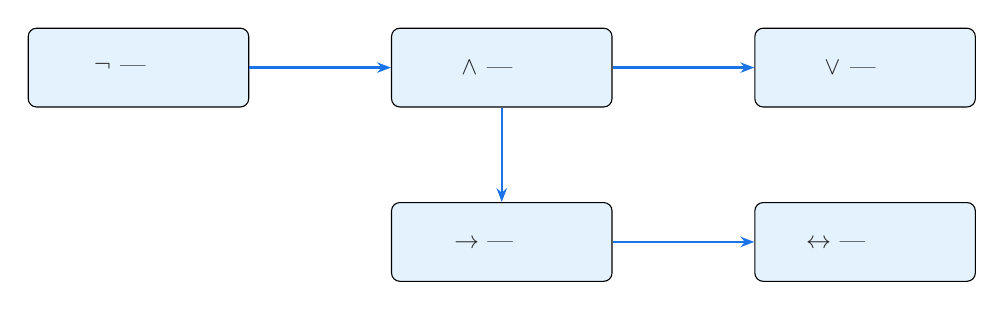
\begin{tikzpicture}[
  node distance=1.8cm,
  every node/.style={
    draw,rounded corners=3pt,
    minimum width=2.8cm,minimum height=1cm,
    font=\small,fill=TheoremBG,
    text=DarkText
  },
  arr/.style={-{Stealth[length=5pt]},thick,PrimaryBlue}
]
  \node (neg) {$\neg$ — نقیض};
  \node (and) [right=of neg] {$\land$ — عطف};
  \node (or)  [right=of and] {$\lor$ — فصل};
  \node (imp) [below=1.2cm of and] {$\to$ — شرطی};
  \node (iff) [right=of imp] {$\leftrightarrow$ — دو شرطی};

  \draw[arr] (neg) -- (and);
  \draw[arr] (and) -- (or);
  \draw[arr] (and) -- (imp);
  \draw[arr] (imp) -- (iff);
\end{tikzpicture}
\end{center}

\subsection{جدول ارزش کامل}
\label{subsec:truthtable}

\begin{table}[htbp]
  \centering
  \caption{جدول ارزش تمامی عملگرهای دوتایی}
  \label{tab:all-ops}
  \rowcolors{2}{LightBG}{white}
  \begin{tabular}{cc|ccccc}
    \toprule
    \rowcolor{AccentTeal!20}
    $p$ & $q$ & $p\land q$ & $p\lor q$ & $p\to q$
        & $p\leftrightarrow q$ & $p\oplus q$ \\
    \midrule
    T & T & T & T & T & T & F \\
    T & F & F & T & F & F & T \\
    F & T & F & T & T & F & T \\
    F & F & F & F & T & T & F \\
    \bottomrule
  \end{tabular}
\end{table}

\section{تاتولوژی و تناقض}

\begin{definition}{تاتولوژی (Tautology)}{tautology}
  گزاره مرکب $\varphi$ یک \textbf{تاتولوژی} است اگر و تنها اگر
  تحت \emph{هر} تخصیص ارزش، مقدار آن درست ($\top$) باشد:
  $$
    \models \varphi
    \quad\Longleftrightarrow\quad
    \forall\, v : v(\varphi) = \top
  $$
\end{definition}

\begin{theorem}{تاتولوژی بودن $p \lor \neg p$}{lem}
  برای هر گزاره $p$:
  \begin{equation}
    \models\; p \lor \neg p
    \label{eq:lem}
  \end{equation}
  این قضیه به \textbf{اصل طرد شق ثالث}
  (\lr{Law of Excluded Middle}) معروف است.%
  \endnote{اصل طرد شق ثالث در منطق شهودی
    (\lr{Intuitionistic Logic}) پذیرفته نیست.
    برای جزئیات بیشتر \cite{godel1931} را ببینید.}
\end{theorem}

\begin{proofbox}
  دو حالت وجود دارد:
  \begin{itemize}[leftmargin=1.5em]
    \item اگر $p = \top$ آنگاه $p \lor \neg p = \top \lor \bot = \top$.
    \item اگر $p = \bot$ آنگاه $p \lor \neg p = \bot \lor \top = \top$.
  \end{itemize}
  پس در هر دو حالت مقدار درست است. \hfill$\blacksquare$
\end{proofbox}

% ////////////////////////////////////////////////////////////
\chapter{منطق محمولات و اثبات‌های صوری}
\label{chap:predicate}
% ////////////////////////////////////////////////////////////

\section{سورها و محمولات}
\label{sec:quantifiers}

\begin{definition}{سور عمومی و وجودی}{quantifiers}
  \begin{align}
    \forall x\, P(x) &\quad\text{«برای \textbf{هر} $x$، $P(x)$ برقرار است»}
      \label{eq:forall}\\
    \exists x\, P(x) &\quad\text{«\textbf{وجود دارد} $x$ که $P(x)$ برقرار است»}
      \label{eq:exists}
  \end{align}
\end{definition}

\subsection{اثبات صوری به روش استنتاج طبیعی}
\label{subsec:natded}

\begin{theorem}{رابطه سورها (نفی سور عمومی)}{quant-neg}
  \begin{equation}
    \neg \forall x\, P(x) \;\equiv\; \exists x\, \neg P(x)
    \label{eq:quant-neg}
  \end{equation}
\end{theorem}

\begin{proofbox}
  \textbf{اثبات ← (جهت چپ به راست):}

  فرض کنید $\neg\forall x\, P(x)$.
  به‌طور برهان خلف فرض کنید
  $\neg\exists x\,\neg P(x)$.
  آنگاه برای هر $x$ داریم $\neg\neg P(x)$،
  یعنی $P(x)$. پس $\forall x\, P(x)$ که تناقض است.

  \medskip
  \textbf{اثبات → (جهت راست به چپ):}

  فرض کنید $\exists x\,\neg P(x)$.
  پس عنصری مانند $a$ وجود دارد که $\neg P(a)$.
  اگر $\forall x\, P(x)$ برقرار بود آنگاه $P(a)$ که تناقض.
  \hfill$\blacksquare$
\end{proofbox}

\section{درخت اثبات}
\label{sec:prooftree}

زیر یک درخت اثبات (\lr{Proof Tree}) به سبک
\textbf{Gentzen} برای
$\{p \to q,\; q \to r\} \vdash p \to r$
رسم شده:

\begin{center}
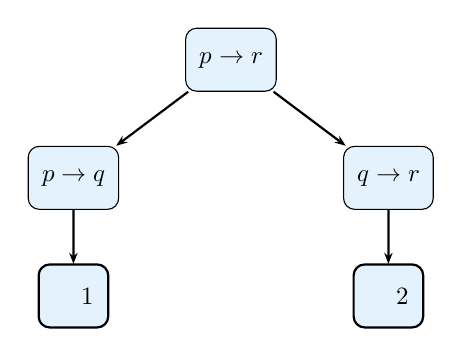
\begin{tikzpicture}[
  level distance=1.5cm,sibling distance=4cm,
  every node/.style={
    draw,rounded corners,fill=TheoremBG,
    minimum height=0.8cm,font=\small,
    inner sep=5pt
  },
  edge from parent/.style={draw,thick,-{Stealth[length=4pt]}}
]
  \node {$p \to r$}
    child {
      node {$p \to q$}
      child { node {فرض $1$} }
    }
    child {
      node {$q \to r$}
      child { node {فرض $2$} }
    };
\end{tikzpicture}
\end{center}

% ============== الگوریتم ===============
\section{الگوریتم بررسی تاتولوژی}
\label{sec:algo}

\begin{algorithm}[H]
  \SetAlgoLined
  \KwIn{فرمول گزاره‌ای $\varphi$ با $n$ متغیر}
  \KwOut{آیا $\varphi$ تاتولوژی است؟}

  \For{$i \leftarrow 0$ \KwTo $2^n - 1$}{
    $v \leftarrow$ تخصیص ارزش متناظر با $i$\;
    \If{$\mathrm{Eval}(\varphi, v) = \bot$}{
      \Return{\textsf{خیر}}\;
    }
  }
  \Return{\textsf{بله}}\;
  \caption{بررسی تاتولوژی با شمارش کامل}
  \label{algo:tautology}
\end{algorithm}

% ////////////////////////////////////////////////////////////
\chapter{نمودارها، تصاویر و جداول}
\label{chap:visuals}
% ////////////////////////////////////////////////////////////

\section{نمودار pgfplots}
\label{sec:pgfplots}

\subsection{نمودار تابع}

\begin{figure}[htbp]
  \centering
  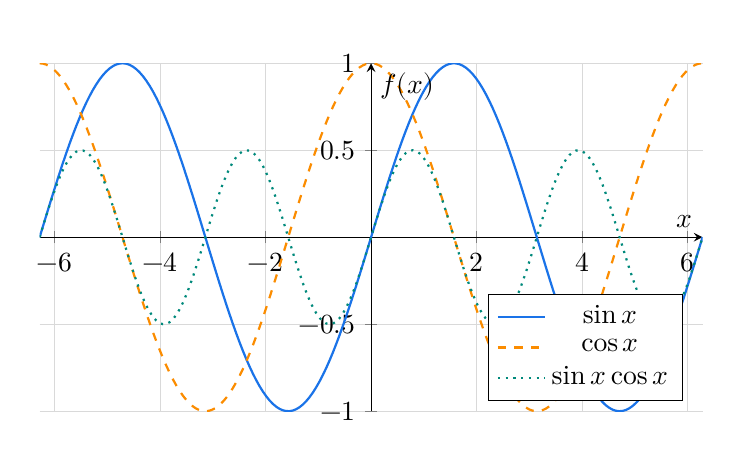
\begin{tikzpicture}
    \begin{axis}[
      width=10cm,height=6cm,
      grid=major,grid style={gray!30},
      xlabel={$x$},ylabel={$f(x)$},
      title={\textbf{نمودار توابع مثلثاتی}},
      title style={font=\large,color=DarkText},
      legend pos=south east,
      axis lines=middle,
      domain=-2*pi:2*pi,samples=200,
      every axis plot/.style={thick}
    ]
      \addplot[PrimaryBlue] {sin(deg(x))};
      \addplot[AccentOrange,dashed] {cos(deg(x))};
      \addplot[AccentTeal,dotted] {sin(deg(x))*cos(deg(x))};
      \legend{$\sin x$, $\cos x$, $\sin x\cos x$}
    \end{axis}
  \end{tikzpicture}
  \caption{نمودار توابع مثلثاتی \lr{(Trigonometric Functions)}}
  \label{fig:trig}
\end{figure}

\subsection{نمودار میله‌ای}

\begin{figure}[htbp]
  \centering
  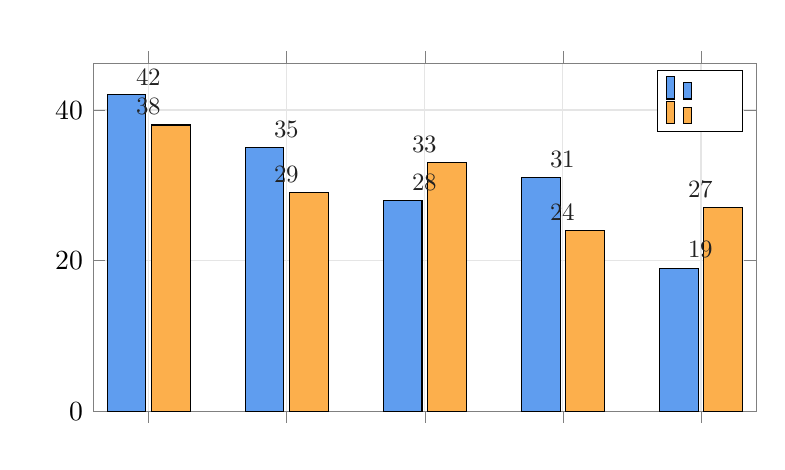
\begin{tikzpicture}
    \begin{axis}[
      ybar,width=10cm,height=6cm,
      bar width=14pt,
      symbolic x coords={منطق,جبر,آنالیز,هندسه,ترکیبیات},
      xtick=data,
      ylabel={تعداد مقاله},
      title={\textbf{مقالات منتشرشده بر حسب شاخه}},
      nodes near coords,
      every node near coord/.style={font=\small,color=DarkText},
      ymin=0,
      axis line style={gray},
      grid=major,grid style={gray!20}
    ]
      \addplot[fill=PrimaryBlue!70] coordinates
        {(منطق,42)(جبر,35)(آنالیز,28)(هندسه,31)(ترکیبیات,19)};
      \addplot[fill=AccentOrange!70] coordinates
        {(منطق,38)(جبر,29)(آنالیز,33)(هندسه,24)(ترکیبیات,27)};
      \legend{۱۴۰۲, ۱۴۰۳}
    \end{axis}
  \end{tikzpicture}
  \caption{مقایسه مقالات منتشرشده در دو سال}
  \label{fig:bar}
\end{figure}

\subsection{نمودار دایره‌ای}

\begin{figure}[htbp]
  \centering
  \begin{tikzpicture}
    \pie[
      text=legend,
      radius=3,
      color={PrimaryBlue!70,AccentTeal!70,AccentOrange!70,
             SidebarGray,ProofBG}
    ]{
      35/منطق کلاسیک,
      25/منطق شهودی,
      20/منطق موجهات,
      12/منطق فازی,
      8/سایر
    }
  \end{tikzpicture}
  \caption{توزیع مقالات بر حسب نوع منطق}
  \label{fig:pie}
\end{figure}
% توجه: برای pie chart باید \usepackage{pgf-pie} اضافه شود
% اگر در دسترس نبود، از tikz خالص رسم کنید

\section{شکل‌های TikZ}
\label{sec:tikzfigs}

\subsection{نمودار ذهنی (\lr{Mind Map})}

\begin{figure}[htbp]
  \centering
  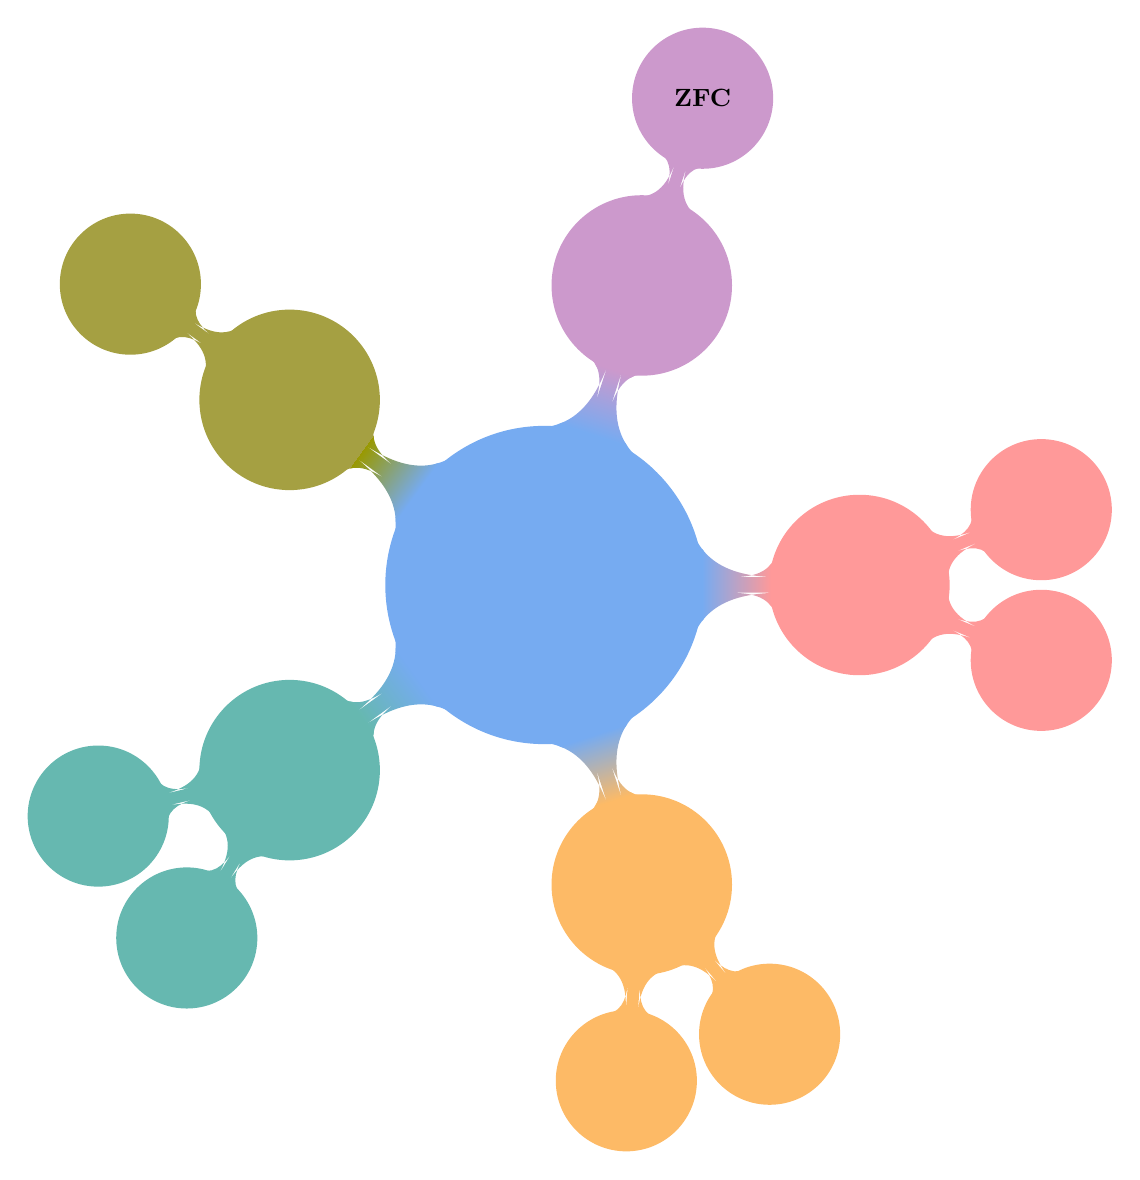
\begin{tikzpicture}[
    mindmap,grow cyclic,
    every node/.style={concept,font=\small\bfseries},
    concept color=PrimaryBlue!60,
    level 1/.append style={level distance=4cm,sibling angle=72},
    level 2/.append style={level distance=2.5cm,sibling angle=45}
  ]
    \node {منطق ریاضی}
      child[concept color=AccentTeal!60] { node {گزاره‌ای}
        child { node {جدول ارزش} }
        child { node {تاتولوژی} }
      }
      child[concept color=AccentOrange!60] { node {محمولات}
        child { node {سورها} }
        child { node {مدل} }
      }
      child[concept color=red!40] { node {اثبات}
        child { node {طبیعی} }
        child { node {تابلو} }
      }
      child[concept color=violet!40] { node {مجموعه‌ها}
        child { node {ZFC} }
      }
      child[concept color=yellow!60!black] { node {بازگشت}
        child { node {تورینگ} }
      };
  \end{tikzpicture}
  \caption{نقشه ذهنی شاخه‌های منطق ریاضی}
  \label{fig:mindmap}
\end{figure}

\subsection{فلوچارت (\lr{Flowchart})}

\begin{figure}[htbp]
  \centering
  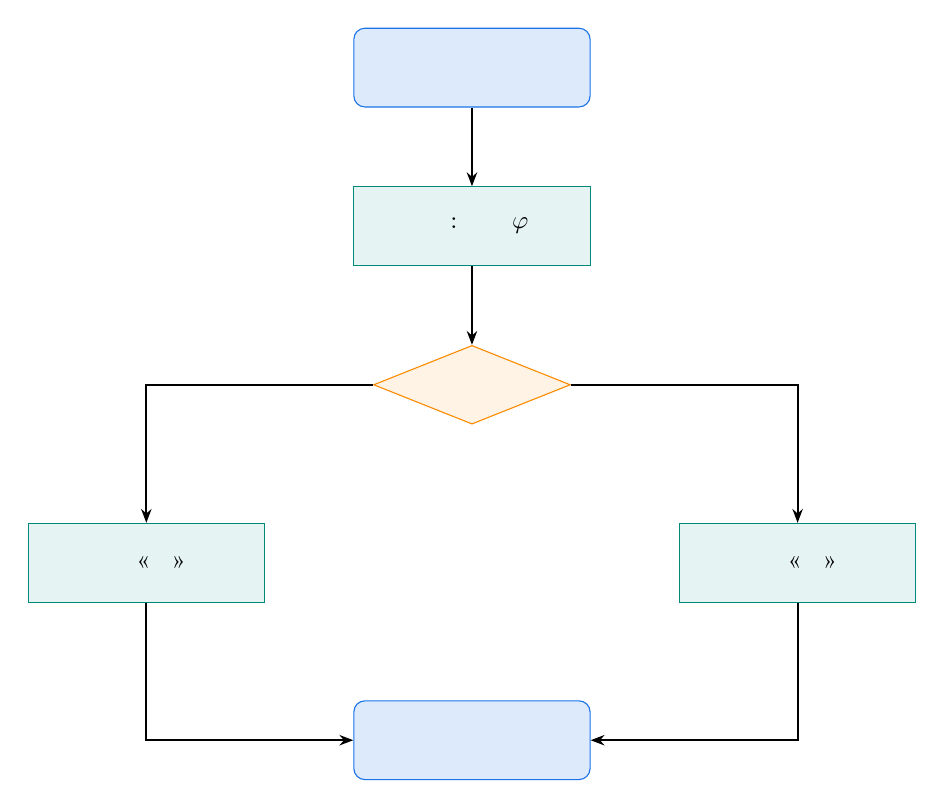
\begin{tikzpicture}[
    startstop/.style={rectangle,rounded corners,
      draw=PrimaryBlue,fill=PrimaryBlue!15,
      minimum width=3cm,minimum height=1cm,font=\small},
    process/.style={rectangle,draw=AccentTeal,fill=AccentTeal!10,
      minimum width=3cm,minimum height=1cm,font=\small},
    decision/.style={diamond,draw=AccentOrange,fill=AccentOrange!10,
      minimum width=2.5cm,minimum height=1cm,
      font=\small,aspect=2},
    arr/.style={-{Stealth[length=5pt]},thick}
  ]
    \node[startstop] (start) {شروع};
    \node[process,below=of start] (input)
      {ورودی: فرمول $\varphi$};
    \node[decision,below=of input] (check)
      {تاتولوژی؟};
    \node[process,below left=1.5cm and 2cm of check] (yes)
      {چاپ «بله»};
    \node[process,below right=1.5cm and 2cm of check] (no)
      {چاپ «خیر»};
    \node[startstop,below=3.5cm of check] (end) {پایان};

    \draw[arr] (start)  -- (input);
    \draw[arr] (input)  -- (check);
    \draw[arr] (check)  -| node[above,pos=0.3]{\small بله} (yes);
    \draw[arr] (check)  -| node[above,pos=0.3]{\small خیر} (no);
    \draw[arr] (yes)    |- (end);
    \draw[arr] (no)     |- (end);
  \end{tikzpicture}
  \caption{فلوچارت الگوریتم بررسی تاتولوژی}
  \label{fig:flowchart}
\end{figure}

\section{تصویر خارجی و \lr{wrapfigure}}
\label{sec:externalimg}

\begin{wrapfigure}{l}{0.35\textwidth}
  \centering
  % چون تصویر واقعی نداریم، از یک جعبه رنگی استفاده می‌کنیم
  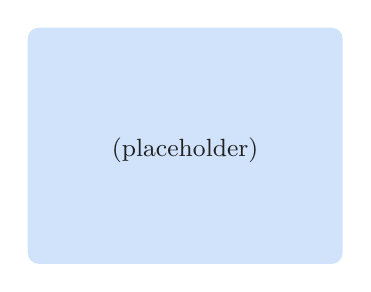
\begin{tikzpicture}
    \fill[PrimaryBlue!20,rounded corners]
      (0,0) rectangle (4,3);
    \node[text=DarkText,font=\small] at (2,1.5)
      {\shortstack{تصویر نمونه\\(placeholder)}};
  \end{tikzpicture}
  \caption{تصویر جایگزین}
  \label{fig:wrap}
\end{wrapfigure}

این متن در کنار تصویر قرار گرفته تا نحوه عملکرد
\lr{wrapfigure} را نشان دهد. در تبدیل به \lr{MDX}
این نوع چیدمان باید حفظ یا به شکل مناسبی
بازنمایی شود. تصاویر کنار متن در مقالات علمی
بسیار رایج‌اند و تبدیل‌گر باید آن‌ها را به‌درستی
به یک \lr{component} مناسب تبدیل کند.
لورم ایپسوم متن ساختگی با تولید سادگی نامفهوم
از صنعت چاپ، و با استفاده از طراحان گرافیک است.

\section{جدول افقی (\lr{Landscape Table})}
\label{sec:landscape}

\begin{sidewaystable}
  \centering
  \caption{جدول افقی — مقایسه سیستم‌های اثبات}
  \label{tab:landscape}
  \rowcolors{2}{LightBG}{white}
  \small
  \begin{tabularx}{\textwidth}{
    >{\bfseries}l
    >{\centering\arraybackslash}X
    >{\centering\arraybackslash}X
    >{\centering\arraybackslash}X
    >{\centering\arraybackslash}X
    >{\centering\arraybackslash}X}
    \toprule
    \rowcolor{PrimaryBlue!20}
    سیستم & نوع & تمامیت & سازگاری & پیچیدگی & ملاحظات \\
    \midrule
    هیلبرت
      & اصل‌موضوعی & بله & بله & بالا
      & تعداد بدیهی زیاد \\
    استنتاج طبیعی
      & قاعده‌محور & بله & بله & متوسط
      & شهودی‌تر \\
    حساب ردیف‌ها (\lr{Sequent})
      & ساختاری & بله & بله & متوسط
      & قاعده برش \\
    تابلو
      & درختی & بله & بله & پایین
      & جستجوی خودکار \\
    رزولوشن
      & مکانیزه & بله (برای CNF) & بله & بالا
      & پایه \lr{SAT Solvers} \\
    \bottomrule
  \end{tabularx}
\end{sidewaystable}

\section{زیرشکل‌ها (\lr{Subfigures})}
\label{sec:subfigs}

\begin{figure}[htbp]
  \centering
  \begin{subfigure}[b]{0.45\textwidth}
    \centering
    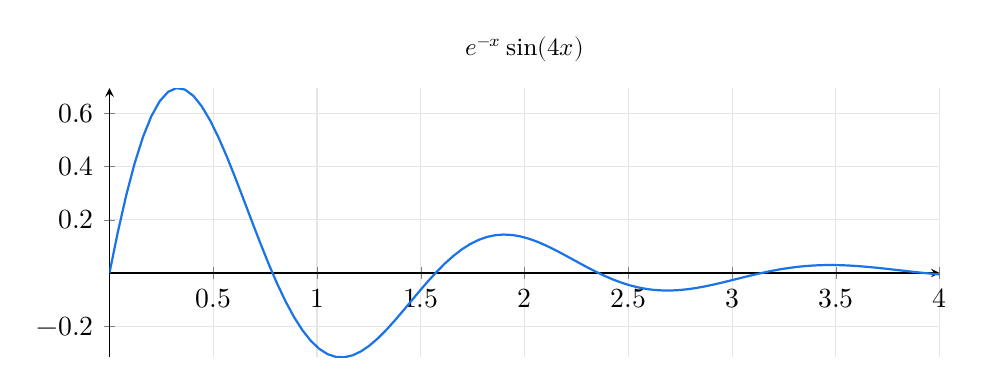
\begin{tikzpicture}
      \begin{axis}[
        width=\textwidth,height=5cm,
        domain=0:4,samples=100,
        title={\small $e^{-x}\sin(4x)$},
        axis lines=middle,grid=major,grid style={gray!20}
      ]
        \addplot[PrimaryBlue,thick]{exp(-x)*sin(deg(4*x))};
      \end{axis}
    \end{tikzpicture}
    \caption{تابع میرا}
    \label{fig:sub1}
  \end{subfigure}
  \hfill
  \begin{subfigure}[b]{0.45\textwidth}
    \centering
    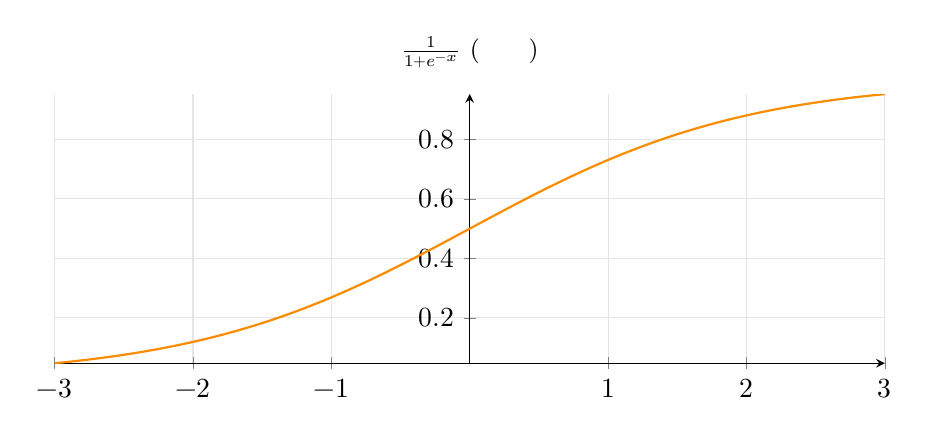
\begin{tikzpicture}
      \begin{axis}[
        width=\textwidth,height=5cm,
        domain=-3:3,samples=100,
        title={\small $\frac{1}{1+e^{-x}}$ (سیگموید)},
        axis lines=middle,grid=major,grid style={gray!20}
      ]
        \addplot[AccentOrange,thick]{1/(1+exp(-x))};
      \end{axis}
    \end{tikzpicture}
    \caption{تابع سیگموید}
    \label{fig:sub2}
  \end{subfigure}
  \caption{مقایسه دو تابع — نمونه زیرشکل}
  \label{fig:subfigs}
\end{figure}

\section{کد برنامه}
\label{sec:code}

\begin{latin}
\begin{lstlisting}[
  language=Python,
  caption={Checking if a formula is a tautology},
  label={lst:python}
]
from itertools import product

def is_tautology(formula, variables):
    """Check if a propositional formula is a tautology."""
    for values in product([True, False], repeat=len(variables)):
        env = dict(zip(variables, values))
        if not formula(env):
            return False
    return True

# Example: p or (not p)
result = is_tautology(
    lambda e: e['p'] or (not e['p']),
    ['p']
)
print(f"p ∨ ¬p is tautology: {result}")  # True
\end{lstlisting}
\end{latin}

\section{فرمول‌های پیچیده ریاضی}
\label{sec:mathformulas}

\subsection{ماتریس‌ها و بردارها}

\begin{equation}
  A = \begin{pmatrix}
    a_{11} & a_{12} & \cdots & a_{1n} \\
    a_{21} & a_{22} & \cdots & a_{2n} \\
    \vdots & \vdots & \ddots & \vdots \\
    a_{m1} & a_{m2} & \cdots & a_{mn}
  \end{pmatrix}
  ,\qquad
  \vec{x} = \begin{pmatrix} x_1 \\ x_2 \\ \vdots \\ x_n \end{pmatrix}
  \label{eq:matrix}
\end{equation}

\subsection{مجموع و انتگرال}

\begin{equation}
  \sum_{k=0}^{\infty} \frac{x^k}{k!} = e^x
  ,\qquad
  \int_{-\infty}^{+\infty} e^{-x^2}\,dx = \sqrt{\pi}
  \label{eq:series-integral}
\end{equation}

\subsection{فرمول‌های چندخطی}

\begin{align}
  \mathcal{L}\{f(t)\} &= \int_{0}^{\infty} e^{-st} f(t)\,dt
    \label{eq:laplace} \\
  \hat{f}(\xi) &= \int_{-\infty}^{+\infty}
    f(x)\,e^{-2\pi i x\xi}\,dx
    \label{eq:fourier} \\
  \nabla \times \mathbf{E} &= -\frac{\partial \mathbf{B}}{\partial t}
    \label{eq:maxwell}
\end{align}

\subsection{حالت‌ها (\lr{cases})}

\begin{equation}
  |x| =
  \begin{cases}
    x  & \text{اگر } x \geq 0 \\
    -x & \text{اگر } x < 0
  \end{cases}
  \label{eq:cases}
\end{equation}

\section{لینک‌ها و ارجاعات متقاطع}

\begin{itemize}[itemsep=4pt]
  \item ارجاع به قضیه: \cref{thm:demorgan}
  \item ارجاع به تعریف: \cref{def:prop}
  \item ارجاع به معادله: \cref{eq:laplace}
  \item ارجاع به شکل: \cref{fig:mindmap}
  \item ارجاع به جدول: \cref{tab:all-ops}
  \item ارجاع به الگوریتم: \cref{algo:tautology}
  \item ارجاع به کد: \cref{lst:python}
  \item لینک خارجی: \href{https://en.wikipedia.org/wiki/Mathematical_logic}{ویکی‌پدیا — منطق ریاضی}
  \item منبع وب: \cite{mdnweb2024}
\end{itemize}

% ////////////////////////////////////////////////////////////
\chapter{راهنمای فنی \lr{\LaTeX} فارسی}
\label{chap:guide}
% ////////////////////////////////////////////////////////////

\begin{warningbox}[⚠ توجه مهم]
  این فصل یک \textbf{مرجع فنی} کامل برای نگارش
  اسناد \lr{\LaTeX} فارسی است و خود بخشی از محتوای
  تست تبدیل فرمت محسوب می‌شود.
\end{warningbox}

\section{پیش‌نیازها و نصب}

\begin{enumerate}[label=\textcolor{PrimaryBlue}{\arabic*.},itemsep=6pt]
  \item \textbf{توزیع تک‌لایو:}
    نسخه کامل \lr{TeX Live 2024} (یا جدیدتر) را نصب کنید.
    روی ویندوز \lr{MiKTeX} نیز قابل استفاده است ولی
    \lr{TeX Live} پیشنهاد می‌شود.

  \item \textbf{کامپایلر:}
    حتماً از \lr{\texttt{xelatex}} استفاده کنید.
    \lr{pdflatex} از فونت‌های فارسی پشتیبانی نمی‌کند.

  \item \textbf{فونت‌ها:}
    فونت‌های زیر را نصب کنید:
    \begin{itemize}
      \item \lr{IRLotus} (یا \lr{XB Niloofar}، \lr{Vazirmatn})
      \item \lr{IranNastaliq} (اختیاری — برای نستعلیق)
      \item یک فونت لاتین مناسب مثل \lr{TeX Gyre Termes}
    \end{itemize}

  \item \textbf{ویرایشگر:}
    \lr{TeXstudio}، \lr{VS Code + LaTeX Workshop}
    یا \lr{Overleaf} پیشنهاد می‌شوند.
\end{enumerate}

\section{ترتیب بارگذاری پکیج‌ها}
\label{sec:pkg-order}

\begin{notebox}[قانون طلایی]
  \texttt{xepersian} \textbf{باید آخرین} پکیج بارگذاری‌شده باشد.
  تنها استثنا پکیج‌هایی هستند که صراحتاً اعلام کرده‌اند
  باید بعد از \lr{xepersian} بیایند (بسیار نادر).
\end{notebox}

ترتیب پیشنهادی:

\begin{latin}
\begin{lstlisting}[language={[LaTeX]TeX},
  caption={ترتیب بارگذاری پکیج‌ها},
  label={lst:pkg-order}]
% 1) Page geometry
\usepackage{geometry}

% 2) Font engine
\usepackage{fontspec}

% 3) Colors (before tikz/tcolorbox)
\usepackage[dvipsnames,svgnames]{xcolor}

% 4) Math
\usepackage{amsmath,amsthm,amssymb,mathtools}
\usepackage{unicode-math}    % optional

% 5) Tables
\usepackage{booktabs,tabularx,longtable,multirow}

% 6) Graphics
\usepackage{graphicx,float,wrapfig}
\usepackage{caption,subcaption}

% 7) TikZ & pgfplots
\usepackage{tikz}
\usepackage{pgfplots}

% 8) Code listings
\usepackage{listings}

% 9) Algorithms
\usepackage[ruled]{algorithm2e}

% 10) Lists
\usepackage{enumitem}

% 11) Hyperref (BEFORE xepersian)
\usepackage[colorlinks]{hyperref}
\usepackage{cleveref}

% 12) Bibliography
\usepackage[backend=biber]{biblatex}

% 13) Headers
\usepackage{fancyhdr}

% === LAST === Persian support
\usepackage[extrafootnotefeatures]{xepersian}
\end{lstlisting}
\end{latin}

\section{تعارضات رایج و راه‌حل}
\label{sec:conflicts}

\begin{longtable}{
    >{\bfseries\small}p{3cm}
    >{\small}p{4.5cm}
    >{\small}p{5.5cm}}
  \caption{تعارضات رایج پکیج‌ها با \lr{xepersian}}
  \label{tab:conflicts} \\
  \toprule
  \rowcolor{PrimaryBlue!15}
  پکیج مشکل‌ساز & مشکل & راه‌حل \\
  \midrule
  \endfirsthead
  \toprule
  \rowcolor{PrimaryBlue!15}
  پکیج & مشکل & راه‌حل \\
  \midrule
  \endhead
  \midrule
  \multicolumn{3}{r}{\small ادامه در صفحه بعد\ldots}\\
  \endfoot
  \bottomrule
  \endlastfoot

  \lr{babel}
    & تداخل مستقیم با \lr{xepersian}
    & هرگز با هم استفاده نکنید \\

  \lr{inputenc}
    & غیرلازم در \lr{XeLaTeX}
    & حذف کنید \\

  \lr{fontenc}
    & تداخل با \lr{fontspec}
    & حذف کنید \\

  \lr{polyglossia}
    & ممکن اما پیچیده
    & ترجیحاً فقط \lr{xepersian} \\

  \lr{hyperref}
    & باید قبل از \lr{xepersian} بیاید
    & ترتیب را رعایت کنید \\

  \lr{cleveref}
    & نیاز به تعریف \lr{crefname} فارسی
    & \lr{\textbackslash crefname} را بازتعریف کنید \\

  \lr{algorithm2e}
    & برخی کلمات کلیدی فارسی نمی‌شوند
    & از \lr{\textbackslash SetKw} استفاده کنید \\

  \lr{listings}
    & مشکل با کاراکترهای یونیکد در کد
    & \lr{literate} تنظیم کنید یا
      \lr{minted} جایگزین \\
\end{longtable}

\section{دستورات کلیدی \lr{xepersian}}
\label{sec:xepersian-cmds}

\begin{table}[htbp]
  \centering
  \caption{دستورات پرکاربرد \lr{xepersian}}
  \label{tab:xepersian-cmds}
  \rowcolors{2}{LightBG}{white}
  \small
  \begin{tabularx}{\textwidth}{lX}
    \toprule
    \rowcolor{AccentTeal!20}
    دستور & توضیح \\
    \midrule
    \lr{\textbackslash settextfont}
      & فونت اصلی متن فارسی \\
    \lr{\textbackslash setlatintextfont}
      & فونت متن لاتین \\
    \lr{\textbackslash setdigitfont}
      & فونت ارقام فارسی \\
    \lr{\textbackslash defpersianfont}
      & تعریف فونت سفارشی فارسی \\
    \lr{\textbackslash lr\{\ldots\}}
      & متن چپ‌به‌راست (لاتین) درون فارسی \\
    \lr{\textbackslash rl\{\ldots\}}
      & متن راست‌به‌چپ (فارسی) درون لاتین \\
    \lr{\textbackslash LTRfootnote}
      & پانوشت انگلیسی \\
    \lr{\textbackslash RTLfootnote}
      & پانوشت فارسی (پیش‌فرض) \\
    \lr{\textbackslash begin\{latin\}}
      & بلوک کامل لاتین \\
    \lr{\textbackslash begin\{persian\}}
      & بازگشت به بلوک فارسی \\
    \lr{\textbackslash twocolumnfootnotes}
      & پانوشت دوستونی \\
    \bottomrule
  \end{tabularx}
\end{table}

\section{نکات تایپوگرافی فارسی}

\begin{enumerate}[label=\textcolor{AccentTeal}{\textbf{\arabic*.}},
  itemsep=6pt]
  \item \textbf{نیم‌فاصله:}
    در ترکیبات فارسی مثل «می‌روم» و «کتاب‌ها» از
    \emph{نیم‌فاصله} (\lr{ZWNJ, U+200C}) استفاده کنید،
    نه فاصله معمولی.

  \item \textbf{گیومه:}
    در فارسی از «\ldots» (گیومه فرانسوی) استفاده کنید
    نه \lr{"..."}.

  \item \textbf{اعداد:}
    با \lr{\textbackslash setdigitfont} ارقام فارسی
    (۰۱۲۳۴۵۶۷۸۹) فعال می‌شوند. در محیط
    \lr{latin} ارقام لاتین نمایش داده می‌شوند.

  \item \textbf{ریاضی:}
    محیط‌های ریاضی (\lr{\$...\$}, \lr{equation},
    \lr{align}) همیشه چپ‌به‌راست هستند و نیاز
    به تنظیم خاصی ندارند.

  \item \textbf{مراجع فارسی:}
    در \lr{biblatex} برای مراجع فارسی از
    \lr{language=persian} استفاده کنید.
\end{enumerate}

\section{فرمان کامپایل}

\begin{latin}
\begin{lstlisting}[language=bash,
  caption={دستورات کامپایل}]
# Compile
xelatex -interaction=nonstopmode document.tex
biber document
xelatex -interaction=nonstopmode document.tex
xelatex -interaction=nonstopmode document.tex

# Or with latexmk (recommended)
latexmk -xelatex -interaction=nonstopmode document.tex
\end{lstlisting}
\end{latin}

% ============================================================
\backmatter
% ============================================================

% ---------- پی‌نوشت‌ها ----------
\theendnotes

% ---------- کتاب‌نامه ----------
\printbibliography[title={کتاب‌نامه}]

\end{document}